\section{Problema de Investigación}

\subsection{Descripción del problema}
Las ciencias exactas, entendida como las ciencias que se basan en la observación y en la experimentación para poder crear conocimientos son las que han permitido comprender muchas de las cosas que pasan en el planeta. Por ello, es obligatorio que en los colegios se den este tipo de ciencias, sin embargo, se evidencia que a los estudiantes se les dificulta el entendimiento de estas asignaturas, además de que les genera un gran temor pues las consideran complejas y casi imposibles de aprender, como es el caso de la asignatura de Física \cite{Solbes2007}.

Esta, a pesar de ser una ciencia elemental, que explica algunos comportamientos del universo y que es de gran relevancia para la educación \cite{CaamanoiRos2011}, en muchas ocasiones el número de horas impartidas de la asignatura en las instituciones no es suficiente para que el estudiante comprenda los conceptos \cite{Rodas2013}. De igual modo, estas pocas horas se basan en clases dirigidas por el docente y, en las cuales solo se dispone de teoría, ejercicios y evaluaciones, metodología que como se dijo anteriormente no funciona ya que los estudiantes siguen con dificultades en su aprendizaje.

De hecho, se evidencia fallas en la implementación de estrategias por parte de las instituciones que permitan motivar y generar mayor curiosidad de los estudiantes hacia el aprendizaje de esta asignatura, generando así que el estudiante estudie sin dinamismo y no dedique tiempo para ella en sus tiempos libres \cite{desinteresEscolar2016}. De igual modo, se reflejan estas fallas debido a que los estudiantes no tienen bases sólidas de conocimientos en materias como las matemáticas, las cuales son fundamentales para la correcta comprensión de asignaturas más complejas como lo es el caso de la física.

En otras palabras, existen factores externos al estudiante como la metodología y horas de clase, que repercuten en lo interno de este como en su motivación que dificultan la comprensión y la solución de problemas de la asignatura Física.

Haciendo énfasis en el caso particular de la Institución Educativa Juan María Céspedes – antes nombrada La Graciela -, para la enseñanza de esta asignatura se dispone solo de los dos últimos años de Bachillerato (diez y once), con una intensidad horaria de tres horas semanales.

Los resultados de las pruebas de validación efectuados a los estudiantes de la Institución Educativa Juan María Céspedes indican que hay un bajo rendimiento en esta asignatura. Para antes del año 2014, cuando la prueba evaluaba individualmente ocho áreas y Física era una de ellas, el comportamiento estadístico del periodo 2011 – 2013 muestra un estancamiento en esta asignatura, obteniendo un resultado en promedio por debajo de 45 puntos [Figura \ref{fig:icfesHis}].

\begin{figure}[H]
    \centering
    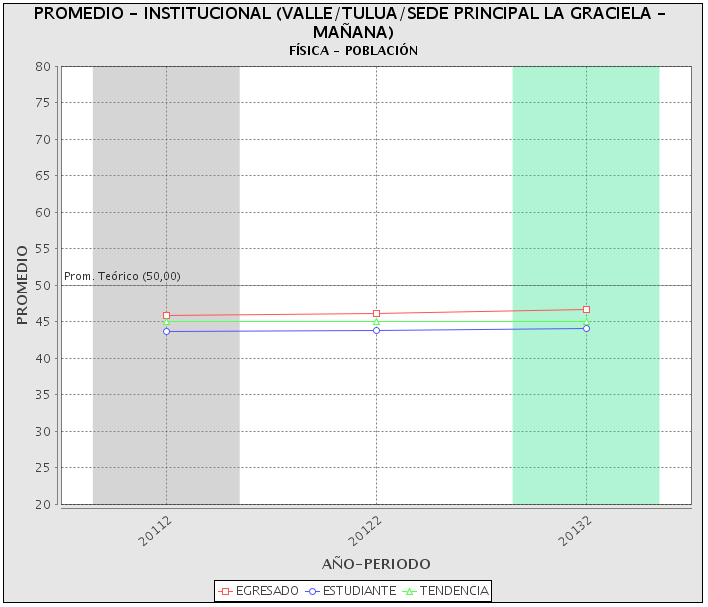
\includegraphics[scale=0.7]{Capitulo_1/imagenes/c0.png}
    \caption{Promedio Pruebas Validación Física Institución Educativa Juan María Céspedes Período 2011-2013}
     \scriptsize \textbf{Fuente:} \cite{icfesHistorico}
    \label{fig:icfesHis}
\end{figure}

Aunque para el año 2014 las pruebas cambiaron y pasaron de ser ocho a ser cinco las áreas a evaluar y Física fuese fusionada junto a Biología y Química en el área de ciencias naturales, se observa que el promedio de los resultados se ha incrementado (50 puntos de 100 posibles), pero no como se esperaría [Figura \ref{fig:icfesProm}].

\begin{table}[H]
    \centering
    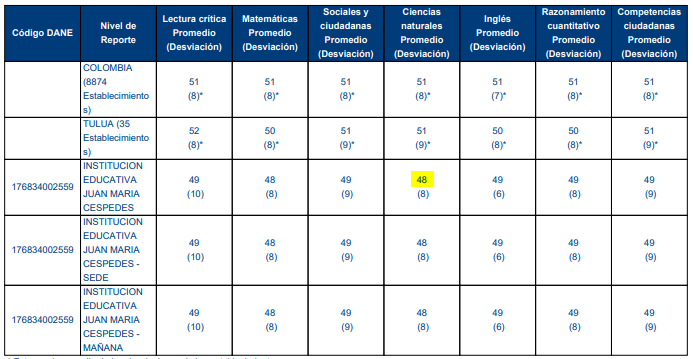
\includegraphics[scale=0.9]{Capitulo_1/imagenes/c1.png}
    \caption{Promedio Pruebas Validación (ICFES) Ciencias Naturales - Año 2014} 
    \scriptsize \textbf{Fuente:} \cite{icfesCiencias}
    \label{tab:icfesNaturales}
\end{table}

\begin{table}[H]
    \centering
    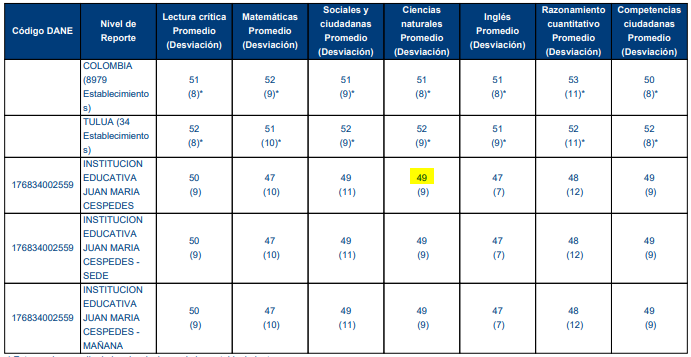
\includegraphics[scale=0.9]{Capitulo_1/imagenes/c2.png}
    \caption{Promedio Pruebas Validación (ICFES) Ciencias Naturales - Año 2015}
    \scriptsize \textbf{Fuente:} \cite{icfesCiencias2}
    \label{tab:icfesNaturales2}
\end{table}

\begin{table}[H]
    \centering
    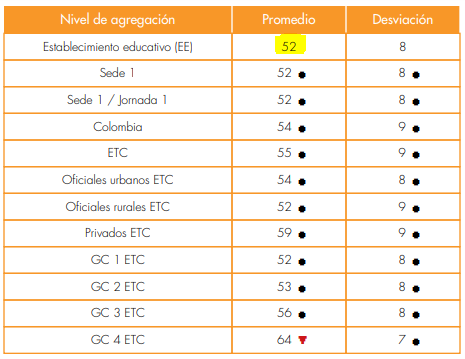
\includegraphics[scale=0.8]{Capitulo_1/imagenes/c3.png}
    \caption{Promedio Pruebas Validación (ICFES) Ciencias Naturales - Año 2016}
    \scriptsize \textbf{Fuente:} \cite{icfesCiencias3}
    \label{tab:icfesNaturales3}
\end{table}

\begin{figure}[H]
    \centering
    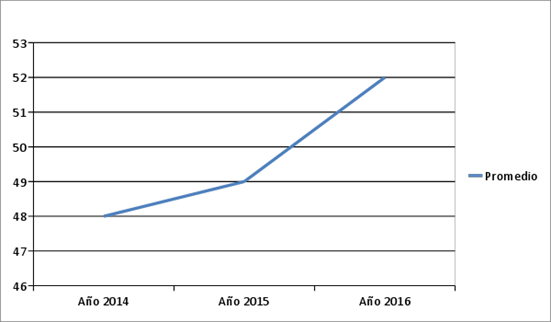
\includegraphics[scale=0.5]{Capitulo_1/imagenes/d5.png}
    \caption{Promedio Pruebas Validación Ciencia Naturales Institución Educativa Juan María Céspedes Período 2014 - 2016}
    \scriptsize \textbf{Fuente:} Elaboración propia
    \label{fig:icfesProm}
\end{figure}


Este bajo rendimiento en física ha planteado el uso de herramientas metodologías que apoyen y faciliten su enseñanza. 

Cabe destacar que una de estas herramientas es el uso de las TIC’s que en los últimos años y en particular en el área de educación, se ha intensificado ya que estas herramientas tecnológicas son más interactivas y logran mantener la atención del estudiante con más facilidad \cite{piedad2014}.

Un ejemplo del uso de estas herramientas tecnológicas en el aula son las aplicaciones hipermedia, que sobresalen por sus amplios beneficios en la enseñanza al brindar una navegación no lineal que atraviesa contenidos o documentos hipertextuales de manera no secuencial, imitando así la complejidad de la mente humana en cuanto a proceso asociativo \cite{Araujo2011}.

Ahora bien, si se tienen en cuenta que en el grado décimo (10$^{\circ}$) inicia la enseñanza de la asignatura física y es donde los estudiantes presentan mayor frustración y mayor temor al enfrentarse por primera vez con ella, es necesario una atención personalizada, donde el estudiante se sienta a gusto en la forma que pueda procesar los contenidos o actividades pertinentes, además de que puede estudiar los temas también desde casa contando con herramientas interactivas que hagan para el estudiante más llamativo y más fácil el contenido de la materia, comprendiendo así, el contenido de la asignatura de una manera más práctica.

\subsection{Formulación del problema}
¿Cómo una aplicación hipermedia puede apoyar el proceso de aprendizaje en la asignatura de Física de los estudiantes del grado 10$^{\circ}$ de la Institución Educativa Juan María Céspedes del municipio de Tuluá, Valle del Cauca?
